\documentclass[12pt]{report}
\usepackage[english, magyar]{babel}
\usepackage{t1enc}
\frenchspacing

\usepackage[margin=2cm, top=5cm, bottom=2.5cm, bindingoffset=0cm]{geometry}
\usepackage{graphicx}

\usepackage{hyperref}
\hypersetup{hidelinks}

\usepackage{xcolor,listings}
\usepackage{textcomp}
\usepackage{color}
\usepackage{listingsutf8}

\definecolor{codegreen}{rgb}{0,0.6,0}
\definecolor{codegray}{rgb}{0.5,0.5,0.5}
\definecolor{codepurple}{HTML}{C42043}
\definecolor{backcolour}{HTML}{F2F2F2}
\definecolor{bookColor}{cmyk}{0,0,0,0.90}  
\definecolor{xmltagcolor}{rgb}{0,0,1}
\definecolor{xmltagcolor}{rgb}{0,0,1}
\definecolor{xmlcommentcolor}{rgb}{0,0.6,0}
\definecolor{xmlstringcolor}{rgb}{0.6,0,0}
\color{bookColor}
\lstset{upquote=true}

\lstdefinestyle{mystyle}{
	language=XML, % Setting the language as XML
	basicstyle=\ttfamily\footnotesize, % Setting the basic style
	morestring=[b]", % Strings are in double quotes
	morestring=[s][\color{xmltagcolor}]{<}{>}, % Coloring XML tags blue
	morecomment=[s][\color{xmlcommentcolor}]{<!--}{-->}, % Coloring comments
	showstringspaces=false, % Not showing spaces in strings
	breaklines=true, % Break long lines
	breakatwhitespace=true, % Break lines at whitespace
	tabsize=2, % Setting tab size
	captionpos=b, % Caption position at bottom
	extendedchars=true, % Allowing extended characters
	keepspaces=true, % Keeping spaces for formatting
}

\lstset{style=mystyle} % Applying the style globally

\usepackage{fancyhdr}
\fancypagestyle{plain}{
\fancyhf{}
\fancyhead[R]{\leftmark}
\fancyhead[L]{\thepage}
\fancyfoot[C]{Adatkezelés XML környezetben}}

\fancyhead[R]{\leftmark}
\fancyhead[L]{\thepage}
\fancyfoot[C]{Adatkezelés XML környezetben}

\begin{document}
	\pagestyle{fancy}
	\title{\Huge JEGYZŐKÖNYV \\ \LARGE Adatkezelés XML környezetben}
	\author{\Large Féléves feladat: Állatkerthálózat}
	\date{\vspace{250px}
		\begin{flushleft}
			Készítette: \textbf{Martinák Mátyás}\\
			Neptunkód: \textbf{KLNSPG}\\
			Dátum: \textbf{2023. 10. 25.}
		\end{flushleft}
		\vspace{15px}
		\begin{center}
			\textbf{Miskolc, 2023}
		\end{center}}
	\maketitle
	
\tableofcontents
\clearpage

\fancyhf{}
\fancyhead[L]{\thepage}

\chapter{A feladat leírása}
A feladat egy vagy több állatkert hálózatát mutatja be, amiben helyet kapnak az egyes állatkertekben dolgozók, azok feladatai, az állatok és élőhelyeik, eledelük, az eledelt gyártó cégek, illetve az állatok örökbefogadói, ha vannak. Mind az ER modell tervezésben és mind az XML megvalósításban angol nyelvet használtam, ugyanis ez a legelterjedtebb nyelv a programozásban\\
Összesen 6 egyedet hoztam létre, melyek a következők:
\begin{itemize}
	\item Employee,
	\item Site,
	\item Habitat,
	\item Animal,
	\item Food,
	\item User
\end{itemize}

\indent Legelőször is érdemes pár szót szólni a \textbf{Site} egyedről. Innen indul ki minden. Ez az egyed tárolja el az egyes
állatkertek legfőbb tulajdonságait, mint pl. név, terület vagy éppen nyitva tartás. Elsődleges kulcsa a \texttt{site\_id}, ami
az állatpark azonosítója.

A Site és az \textbf{Employee} egyed között egy \texttt{1:N} kapcsolat van, mivel egy állatkerthez több dolgozó is tartozhat,
de egy dolgozó, csak egy állatkerthez tartozhat. Az \texttt{1:N} kapcsolat neve: \textbf{Works}. Egy dolgozónak van azonosítója,
vezeték és keresztneve (ami ER modellben egy többágú tulajdonság), neme, születési dátuma és ami a legfontosabb, a dolgozó feladatai, posztjai, amiből lehet egy vagy több, így ez egy többértékű tulajdonság lesz. Ez azért fontos, mivel a relációs modellnél ez a tulajdonság egy külön táblát kap majd, amiben lesz a posztnak egy id-ja, a poszt neve, illetve, hogy kihez tartozik.

Egy állatkerthez több élőhely is tartoztat, de egy élőhely csak egy állatkerthez tartozik. Ezt ábrázolja a \textbf{Manage} kapcsolat, ami \texttt{1:N} kapcsolattal köti össze a Site és a \textbf{Habitat} egyedeket. Az élőhelynek nincsenek ,,extra'' tulajdonságai, van egy azonosítója, neve, térképen való elhelyezkedése, leírása és kapacitása, hogy mennyi állatot
képes egyszerre befogadni.

Az \textbf{Occupy} kapcsolat szintén \texttt{1:N} kapcsolattal köti össze a Habitat-ot az \textbf{Animal}-lel. Az állatnak van azonosítója, neve, faja és leírása.

Itt jön a legelső \texttt{N:M} kapcsolat, az \textbf{Eat}, aminek lesz tulajdonsága, a \texttt{feeding\_time}, az etetési idő. Fontos, hogy megjegyezzük, az \texttt{N:M} kapcsolat külön kapcsolótáblát fog kapni a relációs modellben. Az Eat köti össze az Animalt
a \textbf{Food}-dal, ami az állat eledelét modellező egyed. Ennek van azonosítója, neve, egy \texttt{boolean} (logikai) értéke, ami azt dönti el, hogy finom-e az adott eledel, vagy sem. Ezen kívül van egy többértékű tulajdonsága is, az eledeleket gyártó cégek, amik szintén külön táblát fognak majd kapni a relációs modellben.

Az állatokat örökbe is lehet fogani bizonyos \textbf{User}-eknek, ezt a \textbf{Favor} \texttt{1:1} kapcsolat modellezi. Talán a Usernek
van a legtöbb tulajdonsága ebben az adatbázisban. Van természetesen azonosítója, két neve (vezeték és keresztnév), neme, bejelentkezési adatai (felhasználónév, jelszó), mivel online szeretnénk lebonyolítani az állatok örökbefogadását. Ezen kívül címe is van a felhasználónak, ami az irányítószám, város, utca, házszám tulajdonságokból tevődik össze.

\chapter{I. feladat - XML/XSD létrehozás}

\section[ER modell]{A feladat ER modellje}

\begin{figure}[h]
	\centering
	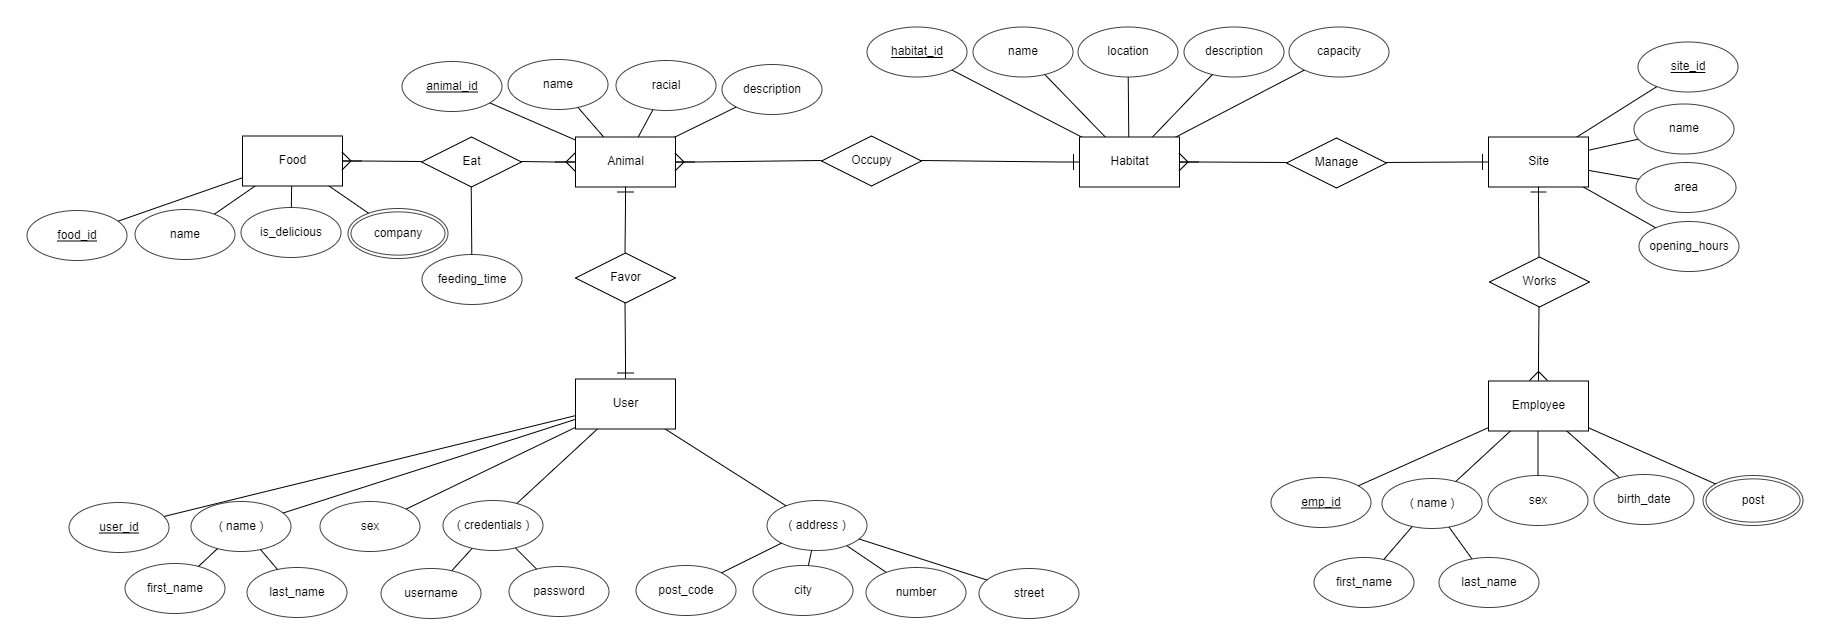
\includegraphics[width=0.999\linewidth]{ERKLNSPG.png}
	\caption{A feladat ER modellje}
\end{figure}

\section[XDM modell]{A feladat XDM modellje}

\indent\indent A konvertáláskor figyelembe kell venni az ER modell során definiált kapcsolatokat, azok típusait (\texttt{1:1, 1:N, N:M}), illetve az entitások elsődleges kulcsait is. Minden \textit{egy-több} kapcsolat esetében ahhoz az elsődleges kulcshoz kerül a szaggatott nyíl, ahol az ER modellben a ,,több'' szerepel. Az ,,Eat'' és a ,,Favor'' kapcsolatokat kivéve, mindenhol \texttt{1:N} kapcsolat szerepel az ER modellben, így az XDM mindenhol majdnem hasonlóan fog kinézni. Az \texttt{N:M} kapcsolat esetében egy új modellt veszünk fel, tulajdonsággal és \textit{primary key}-el együtt természetesen, ahonnan a nyilakat a fő entitásokhoz húzzuk. A többágú tulajdonságok itt is több tulajdonsággal rendelkeznek, a többértékű tulajdonságok itt nem kapnak külön modellt. Az XDM modell gyökéreleme: \textbf{Zoo\_KLNSPG}

\begin{figure}[h]
	\centering
	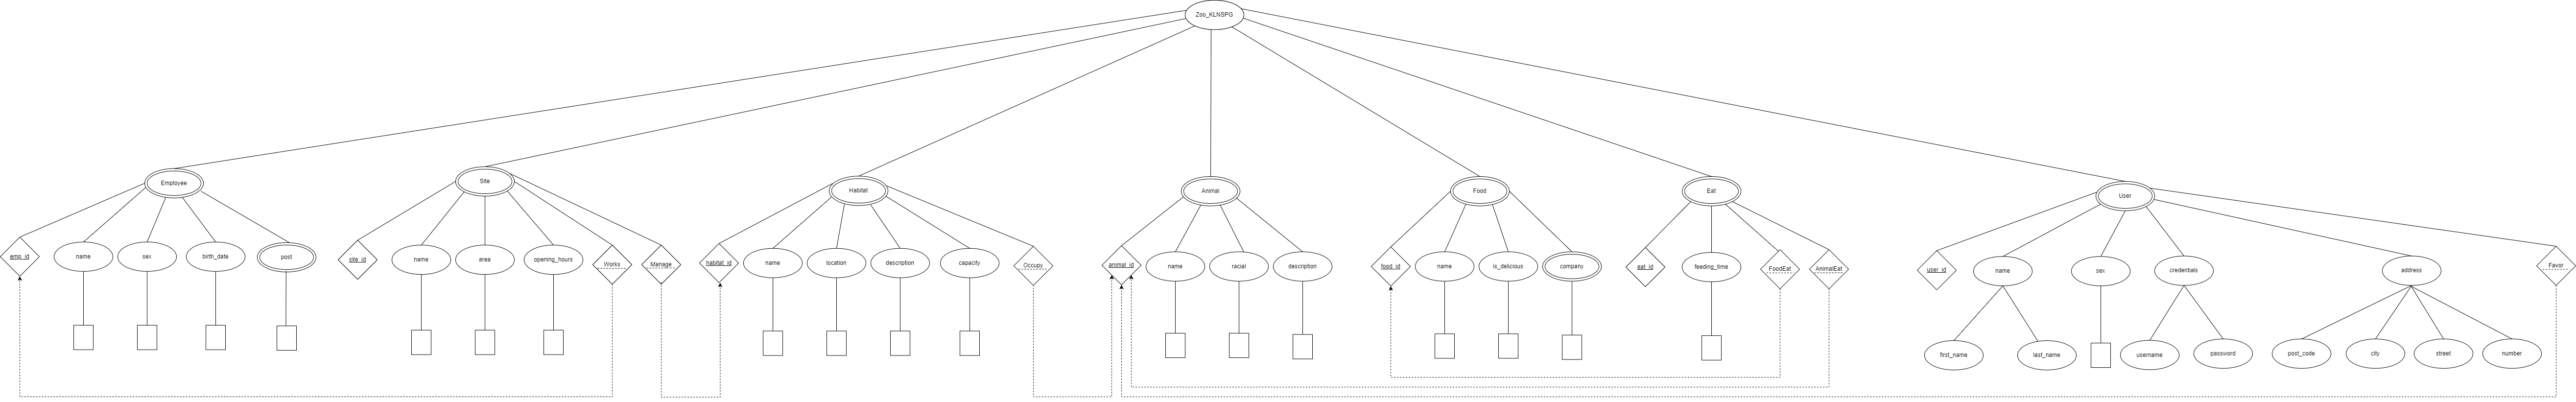
\includegraphics[width=1.01\linewidth]{XDMKLNSPG.png}
	\caption{A feladat XDM modellje}
\end{figure}

A ,,Works'' kapcsolat \texttt{1:N}, ahol a több érték az \textit{Employee}-hoz kerül, így a kapcsolatot is az \textit{emp\_id}-hez húzzuk. Szintén ugyan ez a helyzet a ,,Manage'' kapcsolatnál is, ahol a rombuszt a \textit{habitat\_id}-hoz húzzuk. Az \textit{Animal} modell egy különleges, ide 3 kapcsolatot is húzunk, melyek:

\begin{itemize}
	\item ,,Manage'' a \textit{Habitat}-ból
	\item ,,AnimalEat'' az \textit{Eat}-ből és végül
	\item ,,Favor'' a \textit{User}-ből 
\end{itemize}
Kettő \texttt{1:N} kapcsolat és egy \texttt{1:1} kapcsolat húz ide.

\section[Az XML dokumentum]{Az XDM modell alapján XML dokumentum készítése}
\indent\indent Az \texttt{XMLKLNSPG.xml} dokumentumot \textit{Visual Studio Code}-ban hoztam létre, és \texttt{XML 1.0} szabvány szerint készült el. A dokumentumhoz hozzá kötöttem az \texttt{XMLSchemaKLNSPG.xsd} XSD file-t, és definiáltam az egyedeket az XML szabályainak megfelelően. Ahol szükséges volt, gyermek elemeket, valamint attribútumokat használtam a tagok azonosításához.

\begin{lstlisting}[caption={Az XML dokumentum}]
	<?xml version="1.0" encoding="UTF-8"?>
	
	<Zoo_KLNSPG xmlns:xsi="http://www.w3.org/2001/XMLSchema-instance" xsi:noNamespaceSchemaLocation="XMLSchemaKLNSPG.xsd">
	
	<!-- Employee peldanyok-->
	<Employee emp_id="1">
		<first_name>Kovacs</first_name>
		<last_name>Janos</last_name>
		<birth_date>1979-11-02</birth_date>
		<sex>M</sex>
	</Employee>
	<Employee emp_id="2">
		<first_name>Jakab</first_name>
		<last_name>Jozsef</last_name>
		<birth_date>1954-12-06</birth_date>
		<sex>M</sex>
	</Employee>
		<Employee emp_id="3">
		<first_name>Balogh</first_name>
		<last_name>Boglarka</last_name>
		<birth_date>2000-11-04</birth_date>
		<sex>F</sex>
	</Employee>
	
	<!-- Site peldanyok-->
	<Site site_id="1" Works="3" Manage="1">
		<name>Miskolc Allatkert</name>
		<area>212000</area>
		<opening_hours>09:00 - 17:00</opening_hours>
	</Site>
	<Site site_id="2" Works="1" Manage="2">
		<name>Fovarosi Allat-es Novenykert</name>
		<area>184001</area>
		<opening_hours>09:00 - 17:30</opening_hours>
	</Site>
	<Site site_id="3" Works="2" Manage="3">
		<name>Debreceni Allatkert es Vidampark</name>
		<area>170000</area>
		<opening_hours>09:00 - 15:30</opening_hours>
	</Site>
	
	<!-- Habitat peldanyok-->
	<Habitat habitat_id="1" Occupy="3">
		<name>Medve park</name>
		<location>#3</location>
		<description>Az allatkerti medvek elohelye. Jelenleg harom medve talalhato itt, Jazmin, Andor es Matyko. Szeretik a latogatokat, mindig erdeklodve nezelodnek.</description>
	</Habitat>
	<Habitat habitat_id="2" Occupy="1">
		<name>Muflonok dombja</name>
		<location>#22</location>
		<description>Vadasparkunk muflonjai itt talalhatoak. Baratsagosak, turista kedvelok, szeretik a finom falatokat.</description>
	</Habitat>
	<Habitat habitat_id="3" Occupy="2">
		<name>Szurikatak szigete</name>
		<location>#18</location>
		<description>Ki ne imadna a kis erdeklodo szurikatakat. Nalunk rogton 4-et is orokbe fogadhat, vagy csak latogathat is.</description>
	</Habitat>
	
	<!-- Animal peldanyok-->
	<Animal animal_id="1">
		<name>Matyko</name>
		<racial>Medve</racial>
		<description>Az allatkert egyik kan medveje</description>
	</Animal>
	<Animal animal_id="2">
		<name>Kis Hegyes</name>
		<racial>Muflon</racial>
		<description>Az allatkert nosteny muflona</description>
	</Animal>
		<Animal animal_id="3">
		<name>Mokas</name>
		<racial>Szurikata</racial>
		<description>Az allatkert legfiatalabb szurikataja</description>
	</Animal>
	
	<!-- Food peldanyok-->
	<Food food_id="1">
		<name>Fagyasztott nyershus</name>
		<is_delicious>false</is_delicious>
		<company>Family Frost</company>
	</Food>
	<Food food_id="2">
		<name>Sargarepa</name>
		<is_delicious>true</is_delicious>
		<company>Magyar Zoldseg</company>
	</Food>
	<Food food_id="3">
		<name>Sult husi</name>
		<is_delicious>true</is_delicious>
		<company>Family Frost</company>
	</Food>
	
	<!-- Eat peldanyok-->
	<Eat eat_id="1" FoodEat="1" AnimalEat="3">
		<feeding_time>09:00:00 18:00:00</feeding_time>
	</Eat>
	<Eat eat_id="2" FoodEat="3" AnimalEat="1">
		<feeding_time>07:00:00 20:00:00</feeding_time>
	</Eat>
	<Eat eat_id="3" FoodEat="2" AnimalEat="2">
		<feeding_time>06:00:00 14:00:00 20:00:00</feeding_time>
	</Eat>    
	
	<!-- User peldanyok-->
	<User user_id="1" Favor="3">
		<username>Allatbarat</username>
		<password>allat123</password>
		<sex>M</sex>
		<first_name>Kiss</first_name>
		<last_name>Sandor</last_name>
		<post_code>8200</post_code>
		<city>Veszprem</city>
		<street>Petofi Sandor utca</street>
		<number>3</number>
	</User>
	<User user_id="2" Favor="1">
		<username>Vadoc</username>
		<password>fegyo02</password>
		<sex>M</sex>
		<first_name>Fegyver</first_name>
		<last_name>Sandor</last_name>
		<post_code>4024</post_code>
		<city>Debrecen</city>
		<street>Kossuth utca</street>
		<number>26</number>
	</User>
	<User user_id="3" Favor="2">
		<username>Possumluvr</username>
		<password>possumlover</password>
		<sex>F</sex>
		<first_name>Kazai</first_name>
		<last_name>Eszter</last_name>
		<post_code>3521</post_code>
		<city>Miskolc</city>
		<street>Uj elet utca</street>
		<number>24</number>
	</User>
	
	</Zoo_KLNSPG>
\end{lstlisting}
\clearpage

\section{Az XML dokumentum alapján XMLSchema készítése}
\indent\indent Az \texttt{XMLSchemaKLNSPG.xsd} séma file leírja mindazon megkötéseket, amelyeknek az XML dokumentumnak meg kell felelnie. Itt definiálunk minden típust, amit az XML file-ban használni szeretnénk, valamint az adatbázis kapcsolatait \texttt{xs:unique} és \texttt{xs:keyref} bejegyzésekkel hozom létre.

\begin{lstlisting}[caption={Az XSD dokumentum}]
<?xml version="1.0" encoding="UTF-8"?>
<xs:schema xmlns:xs="http://www.w3.org/2001/XMLSchema">
	
	<!-- Sajat egyszeru tipusok definialasa -->
	
	<!-- Altalanos sajat tipusok-->
	<xs:element name="name" type="xs:string"/>
	<xs:element name="first_name" type="xs:string"/>
	<xs:element name="last_name" type="xs:string"/>
	<xs:element name="sex" type="sexType"/>
	<xs:element name="description" type="xs:string"/>
	
	<!-- Employee sajat tipus-->
	<xs:element name="birth_date" type="dateType"/>
	
	<!-- Site sajat tipusok-->
	<xs:element name="area" type="xs:integer"/>
	<xs:element name="opening_hours" type="xs:string"/>
	
	<!-- Habitat sajat tipus-->
	<xs:element name="location" type="xs:string"/>
	
	<!-- Animal sajat tipus-->
	<xs:element name="racial" type="xs:string"/>
	
	<!-- Food sajat tipus-->
	<xs:element name="is_delicious" type="xs:boolean"/>
	<xs:element name="company" type="xs:string"/>
	
	<!-- Eat sajat tipus-->
	<xs:element name="feeding_time" type="timeListType"/>
	
	<!-- User sajat tipusok-->
	<xs:element name="username" type="xs:string"/>
	<xs:element name="password" type="xs:string"/>
	<xs:element name="post_code" type="xs:string"/>
	<xs:element name="city" type="xs:string"/>
	<xs:element name="street" type="xs:string"/>
	<xs:element name="number" type="xs:string"/>
	
	<!-- Simple types-->
	<xs:simpleType name="dateType">
		<xs:restriction base="xs:date">
			<xs:minInclusive value="1940-01-01"/>
			<xs:maxInclusive value="2000-12-31"/>
		</xs:restriction>
	</xs:simpleType>
	
	<xs:simpleType name="sexType">
		<xs:restriction base="xs:string">
			<xs:enumeration value="M"/>
			<xs:enumeration value="F"/>
		</xs:restriction>
	</xs:simpleType>
	
	<xs:simpleType name="timeListType">
		<xs:list itemType="xs:time"/>
	</xs:simpleType>
	
	<!-- Complex types-->
	<xs:complexType name="employeeType">
		<xs:sequence>
			<xs:element ref="first_name"/>
			<xs:element ref="last_name"/>
			<xs:element ref="birth_date"/>
			<xs:element ref="sex"/>
		</xs:sequence>
		<xs:attribute name="emp_id" type="xs:integer" use="required"/>
	</xs:complexType>
	
	<xs:complexType name="siteType">
		<xs:sequence>
			<xs:element ref="name"/>
			<xs:element ref="area"/>
			<xs:element ref="opening_hours"/>
		</xs:sequence>
		<xs:attribute name="site_id" type="xs:integer" use="required"/>
		<xs:attribute name="Works" type="xs:integer" use="required"/>
		<xs:attribute name="Manage" type="xs:integer" use="required"/>
	</xs:complexType>
	
	<xs:complexType name="habitatType">
		<xs:sequence>
			<xs:element ref="name"/>
			<xs:element ref="location"/>
			<xs:element ref="description"/>
		</xs:sequence>
		<xs:attribute name="habitat_id" type="xs:integer" use="required"/>
		<xs:attribute name="Occupy" type="xs:integer" use="required"/>
	</xs:complexType>
	
	<xs:complexType name="animalType">
		<xs:sequence>
			<xs:element ref="name"/>
			<xs:element ref="racial"/>
			<xs:element ref="description"/>
		</xs:sequence>
		<xs:attribute name="animal_id" type="xs:integer" use="required"/>
	</xs:complexType>
	
	<xs:complexType name="foodType">
		<xs:sequence>
			<xs:element ref="name"/>
			<xs:element ref="is_delicious"/>
			<xs:element ref="company"/>
		</xs:sequence>
		<xs:attribute name="food_id" type="xs:integer" use="required"/>
	</xs:complexType>
	
	<xs:complexType name="eatType">
		<xs:sequence>
			<xs:element ref="feeding_time"/>
		</xs:sequence>
		<xs:attribute name="eat_id" type="xs:integer" use="required"/>
		<xs:attribute name="FoodEat" type="xs:integer" use="required"/>
		<xs:attribute name="AnimalEat" type="xs:integer" use="required"/>
	</xs:complexType>
	
	<xs:complexType name="userType">
		<xs:sequence>
			<xs:element ref="username"/>
			<xs:element ref="password"/>
			<xs:element ref="sex"/>
			<xs:element ref="first_name"/>
			<xs:element ref="last_name"/>
			<xs:element ref="post_code"/>
			<xs:element ref="city"/>
			<xs:element ref="street"/>
			<xs:element ref="number"/>
		</xs:sequence>
		<xs:attribute name="user_id" type="xs:integer" use="required"/>
		<xs:attribute name="Favor" type="xs:integer" use="required"/>
	</xs:complexType>
	
	<!-- A gyokerelem osszetett tipusa -->
	<xs:complexType name="zooType">
		<xs:sequence>
		<xs:element name="Employee" type="employeeType" minOccurs="3" maxOccurs="unbounded"/>
		<xs:element name="Site" type="siteType" minOccurs="3" maxOccurs="unbounded"/>
		<xs:element name="Habitat" type="habitatType" minOccurs="3" maxOccurs="unbounded"/>
		<xs:element name="Animal" type="animalType" minOccurs="3" maxOccurs="unbounded"/>
		<xs:element name="Food" type="foodType" minOccurs="3" maxOccurs="unbounded"/>
		<xs:element name="Eat" type="eatType" minOccurs="3" maxOccurs="unbounded"/>
		<xs:element name="User" type="userType" minOccurs="3" maxOccurs="unbounded"/>
		</xs:sequence>
	</xs:complexType>
	
	<!-- A gyokerelem definicioja -->
	<xs:element name="Zoo_KLNSPG" type="zooType">
	
	<!-- Elsodleges kulcsok -->
	<xs:key name="EmployeeKey">
		<xs:selector xpath="Employee"/>
		<xs:field xpath="@emp_id"/>
	</xs:key>
	
	<xs:key name="SiteKey">
		<xs:selector xpath="Site"/>
		<xs:field xpath="@site_id"/>
	</xs:key>
	
	<xs:key name="HabitatKey">
		<xs:selector xpath="Habitat"/>
		<xs:field xpath="@habitat_id"/>
	</xs:key>
	
	<xs:key name="AnimalKey">
		<xs:selector xpath="Animal"/>
		<xs:field xpath="@animal_id"/>
	</xs:key>
	
	<xs:key name="FoodKey">
		<xs:selector xpath="Food"/>
		<xs:field xpath="@food_id"/>
	</xs:key>
	
	<xs:key name="EatKey">
		<xs:selector xpath="Eat"/>
		<xs:field xpath="@eat_id"/>
	</xs:key>
	
	<xs:key name="UserKey">
		<xs:selector xpath="User"/>
		<xs:field xpath="@user_id"/>
	</xs:key>
	
	<!-- Idegen kulcsok -->
	<xs:keyref name="SiteWork" refer="EmployeeKey">
		<xs:selector xpath="Site"/>
		<xs:field xpath="@Works"/>
	</xs:keyref>
	
	<xs:keyref name="SiteManage" refer="HabitatKey">
		<xs:selector xpath="Site"/>
		<xs:field xpath="@Manage"/>
	</xs:keyref>
	
	<xs:keyref name="HabitatOccupy" refer="AnimalKey">
		<xs:selector xpath="Habitat"/>
		<xs:field xpath="@Occupy"/>
	</xs:keyref>
	
	<xs:keyref name="EatFood" refer="FoodKey">
		<xs:selector xpath="Eat"/>
		<xs:field xpath="@FoodEat"/>
	</xs:keyref>
	
	<xs:keyref name="EatAnimal" refer="AnimalKey">
		<xs:selector xpath="Eat"/>
		<xs:field xpath="@AnimalEat"/>
	</xs:keyref>
	
	<xs:keyref name="UserAnimal" refer="AnimalKey">
		<xs:selector xpath="User"/>
		<xs:field xpath="@Favor"/>
	</xs:keyref>
	
	<!-- Az 1:1 kapcsolat-->
	<xs:unique name="UserAnimalConnect">
		<xs:selector xpath="UserKey"/>
		<xs:field xpath="@Favor"/>
	</xs:unique>
	
	</xs:element>
</xs:schema>
\end{lstlisting}

\chapter{II. feladat - DOM}
\section{Adatolvasás}
\indent\indent A kód egy Java alapú XML feldolgozó program, amely a DOM (Document Object Model) parserét használja. A DOM parser a teljes XML dokumentumot memóriába tölti, ami gyors hozzáférést biztosít az elemekhez, de nagyobb dokumentumok esetén jelentős memóriaigényt jelenthet. A program beolvassa az XML fájlt, normalizálja azt, és különböző függvények segítségével feldolgozza az XML elemeket, melyek az 'Employees', 'Sites', 'Habitats'. Minden elemcsoport feldolgozása külön függvényben történik, ami javítja a kód olvashatóságát és karbantarthatóságát. Hibakezelés is implementálva van a fájlbeolvasás és parse-lás során.\\

\begin{lstlisting}[caption={DOMReadKLNSPG.java} olvasó program, language=Java]
	import javax.xml.parsers.*;
	import org.xml.sax.SAXException;
	import org.w3c.dom.*;
	import java.io.*;
	
	public class DOMReadKLNSPG
	{
		// Main metódus
		public static void main(String[] args) 
		{
			try 
			{
				DocumentBuilderFactory factory = DocumentBuilderFactory.newInstance();
				DocumentBuilder builder = factory.newDocumentBuilder();
				Document document = builder.parse(new File("C:\\projects\\KLNSPG_XMLGyak\\XMLTaskKLNSPG\\XMLKLNSPG.xml"));
				
				document.getDocumentElement().normalize();
				System.out.println("<?xml version=\"1.0\" encoding=\"UTF-8\"?>\n");
				System.out.println("<Zoo_KLNSPG xmlns:xsi=\"http://www.w3.org/2001/XMLSchema-instance\" xsi:noNamespaceSchemaLocation=\"XMLSchemaKLNSPG.xsd\">\n");
				
				readEmployees(document);
				readSites(document);
				readHabitats(document);
				readAnimals(document);
				readFoods(document);
				readEats(document);
				readUsers(document);
				
				System.out.println("\n</Zoo_KLNSPG>");
			} 
			catch (ParserConfigurationException | IOException | SAXException e)
			{
				e.printStackTrace();
			}
		}
		
		// Employee Node beolvasó metódus
		private static void readEmployees(Document document) 
		{
			NodeList employeeList = document.getElementsByTagName("Employee");
			for (int temp = 0; temp < employeeList.getLength(); temp++) 
			{
				Node node = employeeList.item(temp);
				if (node.getNodeType() == Node.ELEMENT_NODE) 
				{
					Element eElement = (Element) node;
					String empId = eElement.getAttribute("emp_id");
					String firstName = eElement.getElementsByTagName("first_name").item(0).getTextContent();
					String lastName = eElement.getElementsByTagName("last_name").item(0).getTextContent();
					String sex = eElement.getElementsByTagName("sex").item(0).getTextContent();
					
					System.out.println("    <Employee emp_id=\"" + empId + "\">");
					printElement("first_name", firstName);
					printElement("last_name", lastName);
					printElement("sex", sex);
					System.out.println("    </Employee>");
				}
			}
		}
		
		// Site Node beolvasó metódus
		private static void readSites(Document document) 
		{
			NodeList siteList = document.getElementsByTagName("Site");
			for (int temp = 0; temp < siteList.getLength(); temp++) 
			{
				Node node = siteList.item(temp);
				if (node.getNodeType() == Node.ELEMENT_NODE) 
				{
					Element eElement = (Element) node;
					String siteId = eElement.getAttribute("site_id");
					String works = eElement.getAttribute("Works");
					String manage = eElement.getAttribute("Manage");
					String name = eElement.getElementsByTagName("name").item(0).getTextContent();
					String area = eElement.getElementsByTagName("area").item(0).getTextContent();
					String openingHours = eElement.getElementsByTagName("opening_hours").item(0).getTextContent();
					
					System.out.println("    <Site site_id=\"" + siteId + "\" Works=\"" + works + "\" Manage=\"" + manage + "\">");
					printElement("name", name);
					printElement("area", area);
					printElement("opening_hours", openingHours);
					System.out.println("    </Site>");
				}
			}
		}
		
		// Habitat Node beolvasó metódus
		private static void readHabitats(Document document) 
		{
			NodeList habitatList = document.getElementsByTagName("Habitat");
			for (int temp = 0; temp < habitatList.getLength(); temp++) 
			{
				Node node = habitatList.item(temp);
				if (node.getNodeType() == Node.ELEMENT_NODE) 
				{
					Element eElement = (Element) node;
					String habitatId = eElement.getAttribute("habitat_id");
					String occupy = eElement.getAttribute("Occupy");
					String name = eElement.getElementsByTagName("name").item(0).getTextContent();
					String location = eElement.getElementsByTagName("location").item(0).getTextContent();
					String description = eElement.getElementsByTagName("description").item(0).getTextContent();
					
					System.out.println("    <Habitat habitat_id=\"" + habitatId + "\" Occupy=\"" + occupy + "\">");
					printElement("name", name);
					printElement("location", location);
					printElement("description", description);
					System.out.println("    </Habitat>");
				}
			}
		}
		
		// Animal Node beolvasó metódus
		private static void readAnimals(Document document) 
		{
			NodeList animalList = document.getElementsByTagName("Animal");
			for (int temp = 0; temp < animalList.getLength(); temp++) 
			{
				Node node = animalList.item(temp);
				if (node.getNodeType() == Node.ELEMENT_NODE) 
				{
					Element eElement = (Element) node;
					String animalId = eElement.getAttribute("animal_id");
					String name = eElement.getElementsByTagName("name").item(0).getTextContent();
					String racial = eElement.getElementsByTagName("racial").item(0).getTextContent();
					String description = eElement.getElementsByTagName("description").item(0).getTextContent();
					
					System.out.println("    <Animal animal_id=\"" + animalId + "\">");
					printElement("name", name);
					printElement("racial", racial);
					printElement("description", description);
					System.out.println("    </Animal>");
				}
			}
		}
		
		// Food Node beolvasó metódus
		private static void readFoods(Document document) 
		{
			NodeList foodList = document.getElementsByTagName("Food");
			for (int temp = 0; temp < foodList.getLength(); temp++) 
			{
				Node node = foodList.item(temp);
				if (node.getNodeType() == Node.ELEMENT_NODE) 
				{
					Element eElement = (Element) node;
					String foodId = eElement.getAttribute("food_id");
					String name = eElement.getElementsByTagName("name").item(0).getTextContent();
					String isDelicious = eElement.getElementsByTagName("is_delicious").item(0).getTextContent();
					String company = eElement.getElementsByTagName("company").item(0).getTextContent();
					
					System.out.println("    <Food food_id=\"" + foodId + "\">");
					printElement("name", name);
					printElement("is_delicious", isDelicious);
					printElement("company", company);
					System.out.println("    </Food>");
				}
			}
		}
		
		// Eat Node beolvasó metódus
		private static void readEats(Document document) 
		{
			NodeList eatList = document.getElementsByTagName("Eat");
			for (int temp = 0; temp < eatList.getLength(); temp++) 
			{
				Node node = eatList.item(temp);
				if (node.getNodeType() == Node.ELEMENT_NODE) 
				{
					Element eElement = (Element) node;
					String eatId = eElement.getAttribute("eat_id");
					String foodEat = eElement.getAttribute("FoodEat");
					String animalEat = eElement.getAttribute("AnimalEat");
					String feedingTime = eElement.getElementsByTagName("feeding_time").item(0).getTextContent();
					
					System.out.println("    <Eat eat_id=\"" + eatId + "\" FoodEat=\"" + foodEat + "\" AnimalEat=\"" + animalEat + "\">");
					printElement("feeding_time", feedingTime);
					System.out.println("    </Eat>");
				}
			}
		}
		
		// User Node beolvasó metódus
		private static void readUsers(Document document)
		{
			NodeList userList = document.getElementsByTagName("User");
			for (int temp = 0; temp < userList.getLength(); temp++) 
			{
				Node node = userList.item(temp);
				if (node.getNodeType() == Node.ELEMENT_NODE) 
				{
					Element eElement = (Element) node;
					String userId = eElement.getAttribute("user_id");
					String favor = eElement.getAttribute("Favor");
					String username = eElement.getElementsByTagName("username").item(0).getTextContent();
					String password = eElement.getElementsByTagName("password").item(0).getTextContent();
					String sex = eElement.getElementsByTagName("sex").item(0).getTextContent();
					String firstName = eElement.getElementsByTagName("first_name").item(0).getTextContent();
					String lastName = eElement.getElementsByTagName("last_name").item(0).getTextContent();
					String postCode = eElement.getElementsByTagName("post_code").item(0).getTextContent();
					String city = eElement.getElementsByTagName("city").item(0).getTextContent();
					String street = eElement.getElementsByTagName("street").item(0).getTextContent();
					String number = eElement.getElementsByTagName("number").item(0).getTextContent();
					
					System.out.println("    <User user_id=\"" + userId + "\" Favor=\"" + favor + "\">");
					printElement("username", username);
					printElement("password", password);
					printElement("sex", sex);
					printElement("first_name", firstName);
					printElement("last_name", lastName);
					printElement("post_code", postCode);
					printElement("city", city);
					printElement("street", street);
					printElement("number", number);
					System.out.println("    </User>");
				}
			}
		}
		
		// Elem kiirato metodus
		private static void printElement(String elementName, String content)
		{
			System.out.println("        <" + elementName + ">" + content + "</" + elementName + ">");
		}
	}
\end{lstlisting}

\section{Adatmódosítás}
\indent\indent A következő program megváltoztat egyes információkat az XML dokumentumban. Az alábbi változtatásokat hajtottam végre:

\begin{itemize}
	\item Az \textit{Employee} példányok elsődleges kulcsának átírása
	\item A Site példányokhoz egy ún. \texttt{visitor\_capacity} attribútum hozzáadása
	\item A \textit{Medve} nevű állat leírásának módosítása
\end{itemize}

\begin{lstlisting}[caption={DOMQModifyKLNSPG.java} olvasó program, language=Java]
	import javax.xml.parsers.*;
	import org.w3c.dom.*;
	import java.io.File;
	
	public class DOMModifyKLNSPG {
		public static void main(String argv[])
		{
			try
			{
				File inputFile = new File("C:\\projects\\KLNSPG_XMLGyak\\XMLTaskKLNSPG\\XMLKLNSPG.xml");
				
				DocumentBuilderFactory docFactory = DocumentBuilderFactory.newInstance();
				DocumentBuilder docBuilder = docFactory.newDocumentBuilder();
				Document doc = docBuilder.parse(inputFile);
				
				System.out.println("--Results--");
				
				modifyAndPrintEmployees(doc);
				modifyAndPrintSites(doc);
				modifyAndPrintAnimals(doc);
			} 
			catch (Exception e)
			{
				e.printStackTrace();
			}
		}
		
		private static void modifyAndPrintEmployees(Document doc)
		{
			NodeList employeeList = doc.getElementsByTagName("Employee");
			for (int i = 0; i < employeeList.getLength(); i++)
			{
				Node employee = employeeList.item(i);
				Element eElement = (Element) employee;
				String empId = eElement.getAttribute("emp_id");
				eElement.setAttribute("emp_id", "EMP_" + empId);
				System.out.println("    Employee {emp_id=" + eElement.getAttribute("emp_id") + "} start");
				printElement("first_name", eElement.getElementsByTagName("first_name").item(0).getTextContent());
				printElement("last_name", eElement.getElementsByTagName("last_name").item(0).getTextContent());
				System.out.println("    Employee end");
			}
		}
		
		private static void modifyAndPrintSites(Document doc)
		{
			NodeList siteList = doc.getElementsByTagName("Site");
			for (int i = 0; i < siteList.getLength(); i++)
			{
				Node site = siteList.item(i);
				Element eElement = (Element) site;
				eElement.setAttribute("visitor_capacity", "5000");
				System.out.println("    Site {visitor_capacity=" + eElement.getAttribute("visitor_capacity") + "} start");
				printElement("name", eElement.getElementsByTagName("name").item(0).getTextContent());
				System.out.println("    Site end");
			}
		}
		
		private static void modifyAndPrintAnimals(Document doc)
		{
			NodeList animalList = doc.getElementsByTagName("Animal");
			for (int i = 0; i < animalList.getLength(); i++)
			{
				Node animal = animalList.item(i);
				Element eElement = (Element) animal;
				if ("Medve".equals(eElement.getElementsByTagName("racial").item(0).getTextContent()))
				eElement.getElementsByTagName("description").item(0).setTextContent("A medve eros es bator");
				
				System.out.println("    Animal start");
				printElement("name", eElement.getElementsByTagName("name").item(0).getTextContent());
				printElement("racial", eElement.getElementsByTagName("racial").item(0).getTextContent());
				printElement("description", eElement.getElementsByTagName("description").item(0).getTextContent());
				System.out.println("    Animal end");
			}
		}
		
		private static void printElement(String elementName, String content)
		{
			System.out.println("        " + elementName + " start");
			System.out.println("            " + content);
			System.out.println("        " + elementName + " end");
		}
	}
\end{lstlisting}

\section{Adatlekérdezés}
\indent\indent Az alábbi program különböző kritériumok alapján kérdez le információkat az XML programból, attribútumok és mezőértékek alapján. Az alábbi lekérdezések írtam meg:
\begin{itemize}
	\item Lekérdezés a férfi Employee-kre
	\item Lekérdezés a legnagyobb $m^3$-rű Site-ra
	\item Lekérdezés az 1999 után született Employee-kre
	\item Lekérdezés a "Medve park" nevű Habitat description-jére
	\item Lekérdezés a 3. id-jú User lakcímére
\end{itemize}

\begin{lstlisting}[caption={DOMQueryKLNSPG.java} olvasó program, language=Java]
import java.io.*;
import javax.xml.parsers.*;
import org.w3c.dom.*;
import org.xml.sax.SAXException;

public class DOMQueryKLNSPG
{
	public static void main(String argv[]) throws SAXException, IOException, ParserConfigurationException
	{
		File xmlFile = new File("C:\\projects\\KLNSPG_XMLGyak\\XMLTaskKLNSPG\\XMLKLNSPG.xml");
		
		DocumentBuilderFactory factory = DocumentBuilderFactory.newInstance();
		DocumentBuilder dBuilder = factory.newDocumentBuilder();
		
		Document doc = dBuilder.parse(xmlFile);
		doc.getDocumentElement().normalize();
		
		NodeList employeeList = doc.getElementsByTagName("Employee");
		System.out.println("\nEmployees:");
		for (int i = 0; i < employeeList.getLength(); i++)
		{
			Node node = employeeList.item(i);
			if (node.getNodeType() == Node.ELEMENT_NODE)
			{
				Element element = (Element) node;
				String sex = element.getElementsByTagName("sex").item(0).getTextContent();
				if (sex.equals("M"))
				{
					String empId = element.getAttribute("emp_id");
					String firstName = element.getElementsByTagName("first_name").item(0).getTextContent();
					String lastName = element.getElementsByTagName("last_name").item(0).getTextContent();
					String birthDate = element.getElementsByTagName("birth_date").item(0).getTextContent();
					System.out.println("ID: " + empId + ", Name: " + firstName + " " + lastName + ", Birth Date: " + birthDate + ", Sex: " + sex);
				}
			}
		}
		
		NodeList siteList = doc.getElementsByTagName("Site");
		int maxArea = 0;
		String maxAreaSiteId = null;
		String maxAreaSiteName = null;
		for (int i = 0; i < siteList.getLength(); i++)
		{
			Node node = siteList.item(i);
			if (node.getNodeType() == Node.ELEMENT_NODE)
			{
				Element element = (Element) node;
				String siteId = element.getAttribute("site_id");
				String name = element.getElementsByTagName("name").item(0).getTextContent();
				String area = element.getElementsByTagName("area").item(0).getTextContent();
				int currentArea = Integer.parseInt(area);
				if (currentArea > maxArea)
				{
					maxArea = currentArea;
					maxAreaSiteId = siteId;
					maxAreaSiteName = name;
				}
			}
		}
		System.out.println("\nSite with the largest area:");
		System.out.println("Site ID: " + maxAreaSiteId + ", Name: " + maxAreaSiteName + ", Area: " + maxArea);
		
		employeeList = doc.getElementsByTagName("Employee");
		System.out.println("\nEmployees born after 1999:");
		for (int i = 0; i < employeeList.getLength(); i++)
		{
			Node node = employeeList.item(i);
			if (node.getNodeType() == Node.ELEMENT_NODE)
			{
				Element element = (Element) node;
				String birthDate = element.getElementsByTagName("birth_date").item(0).getTextContent();
				String[] birthDateParts = birthDate.split("-");
				int birthYear = Integer.parseInt(birthDateParts[0]);
				if (birthYear > 1999)
				{
					String empId = element.getAttribute("emp_id");
					String firstName = element.getElementsByTagName("first_name").item(0).getTextContent();
					String lastName = element.getElementsByTagName("last_name").item(0).getTextContent();
					System.out.println("ID: " + empId + ", Name: " + firstName + " " + lastName + ", Birth Date: " + birthDate);
				}
			}
		}
		
		NodeList habitatList = doc.getElementsByTagName("Habitat");
		System.out.println("\nDescription of \"Medve Park\":");
		for (int i = 0; i < habitatList.getLength(); i++)
		{
			Node node = habitatList.item(i);
			if (node.getNodeType() == Node.ELEMENT_NODE)
			{
				Element element = (Element) node;
				String name = element.getElementsByTagName("name").item(0).getTextContent();
				if (name.equals("Medve park"))
				{
					String description = element.getElementsByTagName("description").item(0).getTextContent();
					System.out.println("Habitat description: " + description);
				}
			}
		}
		
		NodeList userList = doc.getElementsByTagName("User");
		System.out.println("\nAddress of user_id 3:");
		for (int i = 0; i < userList.getLength(); i++)
		{
			Node node = userList.item(i);
			if (node.getNodeType() == Node.ELEMENT_NODE)
			{
				Element element = (Element) node;
				String userId = element.getAttribute("user_id");
				if (Integer.parseInt(userId) == 3)
				{
					String postCode = element.getElementsByTagName("post_code").item(0).getTextContent();
					String city = element.getElementsByTagName("city").item(0).getTextContent();
					String street = element.getElementsByTagName("street").item(0).getTextContent();
					String number = element.getElementsByTagName("number").item(0).getTextContent();
					System.out.println("User address: " + postCode + " " + city + " " + street + " " + number);
				}
			}
		}
	}
}
\end{lstlisting}

\section{Adatírás}


\begin{lstlisting}[caption={DOMWriteKLNSPG.java} olvasó program, language=Java]
import org.w3c.dom.*;
import org.xml.sax.SAXException;

import javax.xml.parsers.*;
import javax.xml.transform.*;
import javax.xml.transform.dom.DOMSource;
import javax.xml.transform.stream.StreamResult;
import java.io.*;

public class DOMWriteKLNSPG
{
	
	public static void main(String[] args)
	{
		try 
		{
			File inputFile = new File("C:\\projects\\KLNSPG_XMLGyak\\XMLTaskKLNSPG\\XMLKLNSPG.xml");
			DocumentBuilderFactory dbFactory = DocumentBuilderFactory.newInstance();
			DocumentBuilder dBuilder = dbFactory.newDocumentBuilder();
			Document doc = dBuilder.parse(inputFile);
			doc.getDocumentElement().normalize();
			
			printNode(doc.getDocumentElement(), "");
			writeDocumentToFile(doc, "XMLKLNSPG1.xml");
			
			System.out.println("The content has been written to the output file successfully.");
		} catch (SAXException | IOException | ParserConfigurationException | TransformerException e) 
		{
			e.printStackTrace();
		}
	}
	
	private static void printNode(Node node, String indent) 
	{
		if (node.getNodeType() == Node.ELEMENT_NODE) 
		{
			System.out.print(indent + node.getNodeName());
			if (node.hasAttributes()) 
			{
				NamedNodeMap nodeMap = node.getAttributes();
				for (int i = 0; i < nodeMap.getLength(); i++) 
				{
					Node attr = nodeMap.item(i);
					System.out.print(attr.getNodeName() + "=" + attr.getNodeValue() + (i < nodeMap.getLength() - 1 ? ", " : ""));
				}
			}
			
			System.out.println(" start");
			
			NodeList children = node.getChildNodes();
			String childIndent = indent + "    ";
			for (int i = 0; i < children.getLength(); i++) 
			printNode(children.item(i), childIndent);
			
			System.out.println(indent + node.getNodeName() + " end");
		} 
		else if (node.getNodeType() == Node.TEXT_NODE) 
		{
			String content = node.getTextContent().trim();
			if (!content.isEmpty()) 
			System.out.println(indent + content);
		}
	}
	
	private static void writeDocumentToFile(Document doc, String filename) throws TransformerException 
	{
		TransformerFactory transformerFactory = TransformerFactory.newInstance();
		Transformer transformer = transformerFactory.newTransformer();
		transformer.setOutputProperty(OutputKeys.INDENT, "yes");
		DOMSource source = new DOMSource(doc);
		StreamResult result = new StreamResult(new File(filename));
		transformer.transform(source, result);
	}
}
\end{lstlisting}

\end{document}